% Bar Chart - EE-Bruttostromerzeugung 2019

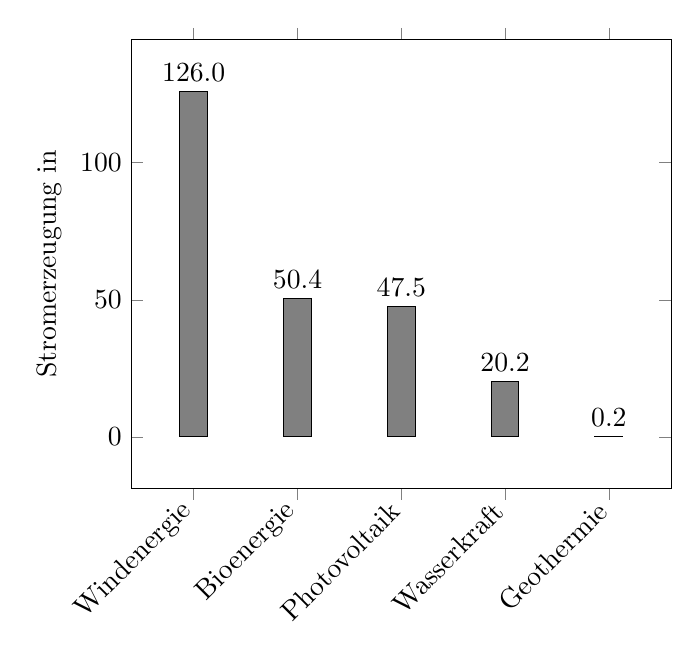
\begin{tikzpicture}
	\begin{axis}[
	ybar,
	enlargelimits=0.15,											% äüßerste bar plots nicht am Limit der x-Achse
	ylabel={Stromerzeugung in \si{\twh}},
	symbolic x coords={Windenergie,
		Bioenergie,
		Photovoltaik,
		Wasserkraft,
		Geothermie 
	},
	xtick=data,
	nodes near coords,											% Zahlen auf den bar plots
	nodes near coords align={vertical},
	nodes near coords style={/pgf/number format/.cd,fixed,fixed zerofill,precision=1},
	x tick label style={rotate=45,anchor=east},
	]
	\addplot[black,fill=black!50!white] coordinates {
		(Windenergie,126.0) (Bioenergie,50.4) (Photovoltaik,47.5) (Wasserkraft,20.2) (Geothermie,0.2)
	};
	\end{axis}
\end{tikzpicture}